\documentclass[ignorenonframetext,xcolor=x11names]{beamer}

\definecolor{mun}{RGB}{134,38,51}
\definecolor{mun2}{RGB}{99,102,106}
%\definecolor{mun}{cmyk}{0,.3922,.2392,.1686}
\definecolor{code}{RGB}{0, 0, 128}
\definecolor{code}{gray}{0.95}

\mode<presentation>
{
%  \usetheme{boxes}
%  \usetheme{default}
%  \usetheme{Montpellier}
%  \usetheme{Singapore}
%   \usetheme{Rochester}
%  \usecolortheme{crane}
%  \usecolortheme{dolphin}
%  \usecolortheme{lily}
%  \usecolortheme{orchid}
  \usecolortheme{rose}
  \setbeamercovered{transparent}
%  \usefonttheme[onlymath]{serif}
  \setbeamercolor*{structure}{bg=mun,fg=mun}
  \setbeamercolor*{palette primary}{use=structure,fg=white,bg=structure.fg}
  \setbeamercolor*{palette secondary}{use=structure,fg=white,bg=structure.fg}
  \setbeamercolor*{palette tertiary}{use=structure,fg=white,bg=black}
  \setbeamercolor*{palette quaternary}{fg=white,bg=black}
  \setbeamercolor{section in toc}{fg=black,bg=white}
  \setbeamercolor{alerted text}{use=structure,fg=structure.fg!50!black!80!black}
  \setbeamercolor{titlelike}{parent=palette primary,fg=structure.fg!50!black}
  \setbeamercolor{frametitle}{bg=mun,fg=white}
  \setbeamercolor*{titlelike}{parent=palette primary}

  \setbeamercolor{normal text}{fg=black!90}
  \setbeamercolor{math text}{fg=black}
  \setbeamercolor{quote}{bg=gray!20}
  \setbeamercolor{quotation}{bg=gray!20}
  \setbeamerfont{cite}{size=\scriptsize}
  \setbeamerfont{quote}{size=\footnotesize}
  \setbeamerfont{quotation}{size=\footnotesize}
  \setbeamercolor{red text}{fg=red!75!black}
  \setbeamertemplate{bibliography item}[triangle]
  \setbeamertemplate{enumerate item}[square]
  \setbeamertemplate{blocks}[rounded][shadow=true]
  \setbeamertemplate{navigation symbols}{}
  \setbeamertemplate{footline}[frame number]
}
\usepackage{tcolorbox}
\usepackage{amsmath}
\usepackage{physics}
\usepackage{pgf}
\usepackage[english]{babel}
\usepackage[latin1]{inputenc}
\usepackage{times}
\usepackage[T1]{fontenc}
\usepackage{multicol}
\usepackage{multirow}
\usepackage{fancyvrb}
\usepackage{tabularx}
\usepackage{amsmath}
\usepackage{bbm}
\usepackage{alltt}
\usepackage{hyperref}
\hypersetup{
    colorlinks=true,
    linkcolor=blue,
    filecolor=magenta,      
    urlcolor=blue,
}
\usepackage{minted}
\newminted{cypher}{autogobble,bgcolor=code,breakbytoken,frame=single,framesep=3pt}
\newminted{R}{autogobble,bgcolor=code,breakbytoken,frame=single,framesep=3pt}
\newminted{text}{autogobble,bgcolor=code,breakbytoken,frame=single,framesep=3pt}
\newminted{sql}{autogobble,bgcolor=code,breakbytoken,frame=single,framesep=3pt}
\newminted{bash}{autogobble,bgcolor=code,breakbytoken,python3,frame=single,framesep=3pt}
\newminted{xml}{autogobble,bgcolor=code,breakbytoken,python3,frame=single,framesep=3pt}
\newminted{python}{bgcolor=code,breakbytoken,python3,frame=single,framesep=3pt}
\newminted{html}{autogobble,bgcolor=code,breakbytoken,frame=single,framesep=3pt}
\newminted{js}{autogobble,bgcolor=code,breakbytoken,frame=single,framesep=3pt}
\AtBeginEnvironment{minted}{%
  \renewcommand{\fcolorbox}[4][]{#4} \scriptsize}
\AtEndEnvironment{minted}{%
  \normalsize}

%\newcommand{\Pr}{\operatorname{Pr}}
\newcommand{\argmax}{\operatorname*{argmax}}
\newcommand{\argmin}{\operatorname*{argmin}}
\newcommand{\Ident}{\operatorname{I}}

\author % (optional, use only with lots of authors)
{Joerg Evermann}
% - Give the names in the same order as the appear in the paper.
% - Use the \inst{?} command only if the authors have different
%   affiliation.

\institute%[Universities of Somewhere and Elsewhere] % (optional, but mostly needed)
{
  Faculty of Business Administration\\
  Memorial University of Newfoundland \\ 
  \texttt{jevermann@mun.ca} 
}

\date{}

\pgfdeclareimage[width=1.5cm]{university-logo}{../MUN_LOGO_CMYK}
\logo{\pgfuseimage{university-logo}}

% If you wish to uncover everything in a step-wise fashion, uncomment
% the following command: 

%\beamerdefaultoverlayspecification{<+->}


\title{Business 4720 - Class 13}

\begin{document}

\begin{frame}{}
  \titlepage
  \footnotesize
  \begin{center}

\includegraphics[height=.5in]{../by-nc.png}

Unless otherwise indicated, the copyright in this material is owned by Joerg Evermann. This material is licensed to you under the \href{https://creativecommons.org/licenses/by-nc/4.0/}{Creative Commons by-attribution non-commercial license (CC BY-NC 4.0)}
\end{center}

\end{frame}

\section{Introduction}

\begin{frame}{This Class}

\begin{block}{What You Will Learn:}
\begin{itemize}
  \item Unsupervised Machine Learning
  \begin{itemize}
     \item Dimension Reduction using Principal Components Analysis
     \item Clustering
  \end{itemize}
\end{itemize}
\end{block}
\end{frame}

\begin{frame}{Based On}
\small
\begin{block}{}
Gareth James, Daniel Witten, Trevor Hastie and Robert Tibshirani: \emph{An Introduction to Statistical Learning with Applications in R}. 2nd edition, corrected printing, June 2023. (ISLR2) \\
\vspace{1mm}
\url{https://www.statlearning.com} \\
\vspace{1mm}
Chapter 12
\end{block}

\begin{block}{}
Trevor Hastie, Robert Tibshirani, and Jerome Friedman: \emph{The Elements of Statistical Learning}. 2nd edition, 12th corrected printing, 2017. (ESL) \\
\vspace{1mm}
\url{https://hastie.su.domains/ElemStatLearn/} \\
\vspace{1mm}
Chapter 14
\end{block}

\begin{block}{}
Kevin P. Murphy: \emph{Probabilistic Machine Learning -- An Introduction}. MIT Press 2022. \\
\vspace{1mm}
\url{https://probml.github.io/pml-book/book1.html} \\
\vspace{1mm}
Chapters 20, 21
\end{block}
\end{frame}

\begin{frame}{Principal Components Analysis (PCA)}
\begin{itemize}
  \item Create linear combinations of predictors that are:
  \begin{itemize}
     \item Maximally variable
     \item Independent of each other
  \end{itemize}
  \item Generally fewer components than predictors
  \item Can be used instead of original predictors in regression or classification models
  \item Useful when the problem dimensionality is too high (too many parameters)
  \begin{itemize}
     \item Can be interpreted as a regularization method
  \end{itemize}
  \item Useful for visualization to show 2D or 3D summaries of high-dimensional data
\end{itemize}
\end{frame}

\begin{frame}{PCA \small [cont'd]}
\begin{columns}
\begin{column}{.7\textwidth}
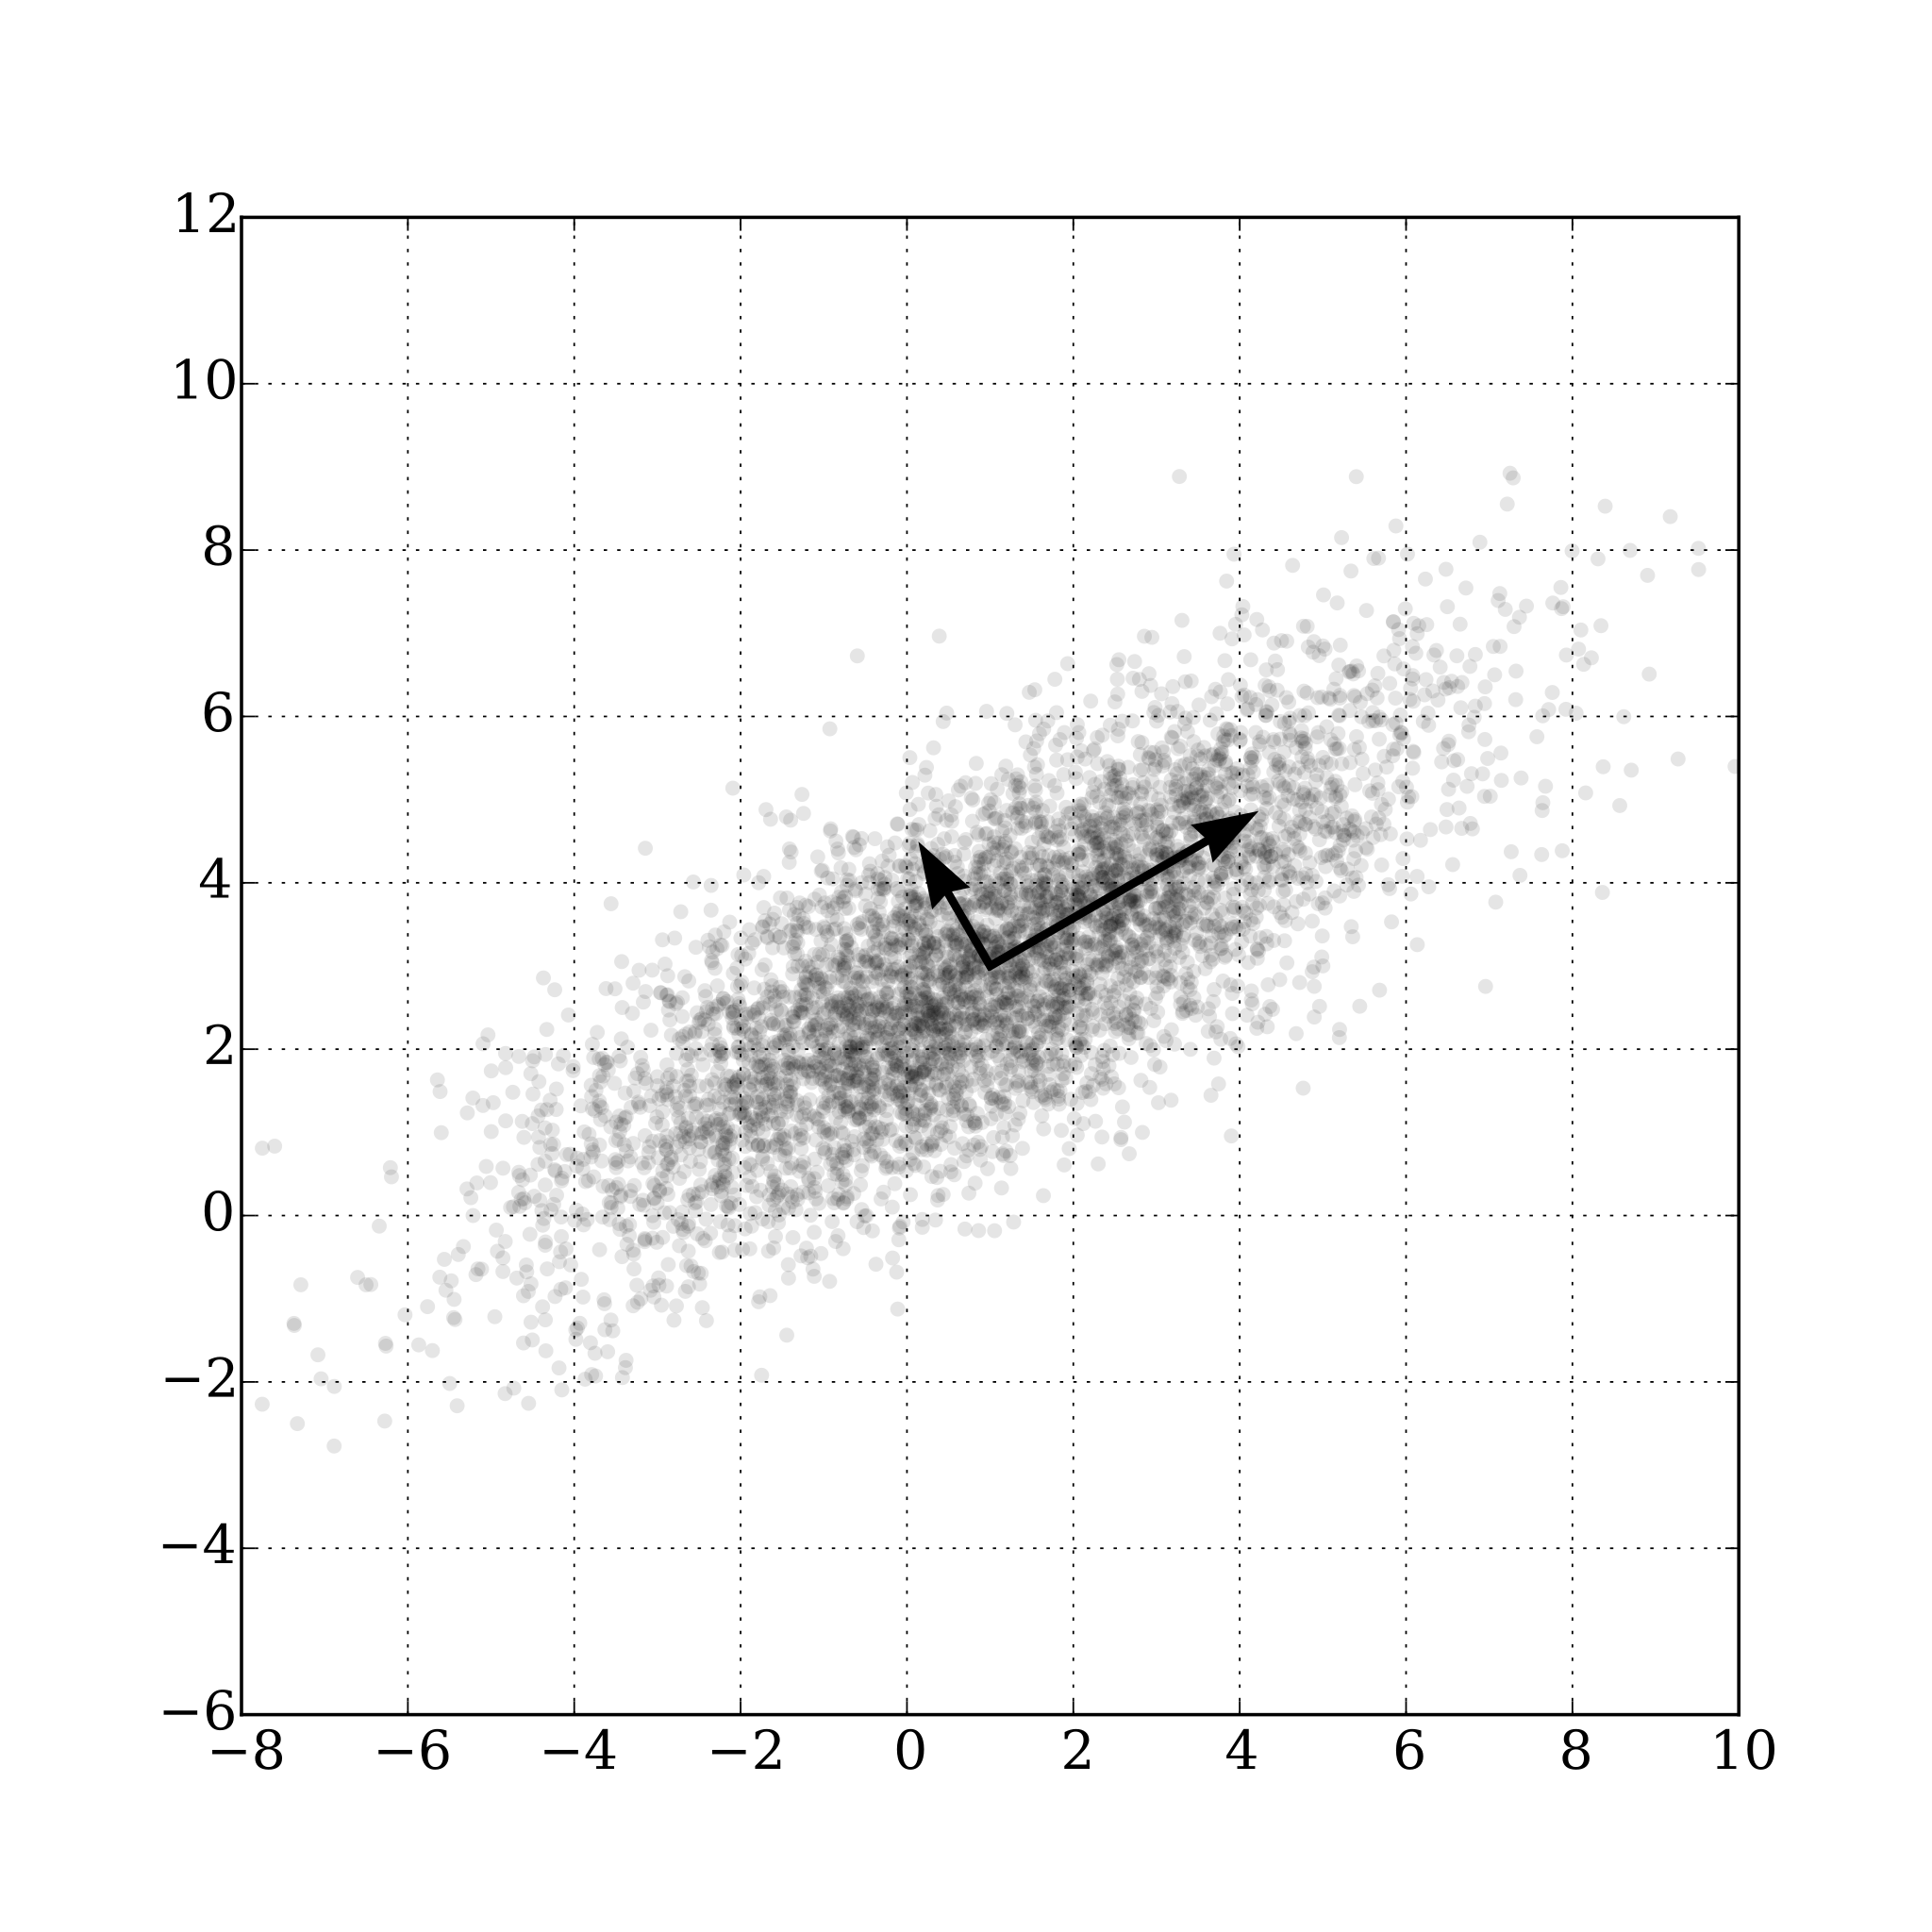
\includegraphics[width=\textwidth]{GaussianScatterPCA.svg.png} \\
\scriptsize
\url{https://commons.wikimedia.org/wiki/File:GaussianScatterPCA.svg} \\
\end{column}
\begin{column}{.3\textwidth}
Scatterplot with \textbf{Principal Components}  \\
\vspace{\baselineskip}
(Eigenvectors of covariance matrix, scaled by the square root of the corresponding eigenvalue and shifted to mean)
\end{column}
\end{columns}
\end{frame}

\begin{frame}{PCA \small [cont'd]}
\begin{itemize}
\item First principal component (PC) for $1 \leq i \leq n$ data values and $p$ variables:
\begin{align*}
z_{i1} = \phi_{11} x_{i1} + \phi_{21} x_{i2} + \cdots + \phi_{p1} x_{ip}
\end{align*}
\item \textbf{Loading vector} $\phi = (\phi_{11}, \ldots , \phi_{p1})$ scaled so that $||\phi||_2 = 1$
\item Assume zero-centered variables
\item Maximize:
\begin{align*}
\frac{1}{n} \sum_{i=1}^n z_{i1}^2 = \frac{1}{n}\sum_{i=1}^n \left( \sum_{j=1}^p \phi_{j1}x_{ij} \right)^2 \qquad \text{(Variance of $z_{i1}$)} 
\end{align*}
\item Subject to:
\begin{align*}
\sum_{j=1}^p \phi_{j1}^2 = 1 \qquad \text{(Scaling constraint)}
\end{align*}
\end{itemize}
\end{frame}

\begin{frame}{PCA \small [cont'd]}
\begin{itemize}
\item For further components $k$, subtract the first $k-1$ components from the data $X$ (residualization), then repeat the maximization
\item At most as many components as data variables $p$
\item Each successive component explains a decreasing proportion of the variance in the data
\item Information loss when using fewer components to represent data
\end{itemize}
\begin{block}{Tips}
\begin{itemize}
  \item Scale data prior to PCA
  \item Principle component signs can be ''flipped'' (arbitrarily)
\end{itemize}
\end{block}
\end{frame}

\begin{frame}{PCA -- Example and Biplot}
\begin{columns}
\begin{column}{0.3\textwidth}
\footnotesize
\begin{tabular}{l|r|r} \hline
          &  PC1 & PC2 \\ \hline
Murder    & .536  & -0.418 \\
Assault   & .583  & -0.188 \\
UrbanPop  & .278  & 0.873 \\ 
Rape      & .543 & 0.167 \\ \hline
\end{tabular} \\

\scriptsize Source: ISLR2 Table 12.1
\end{column}
\begin{column}{0.7\textwidth}
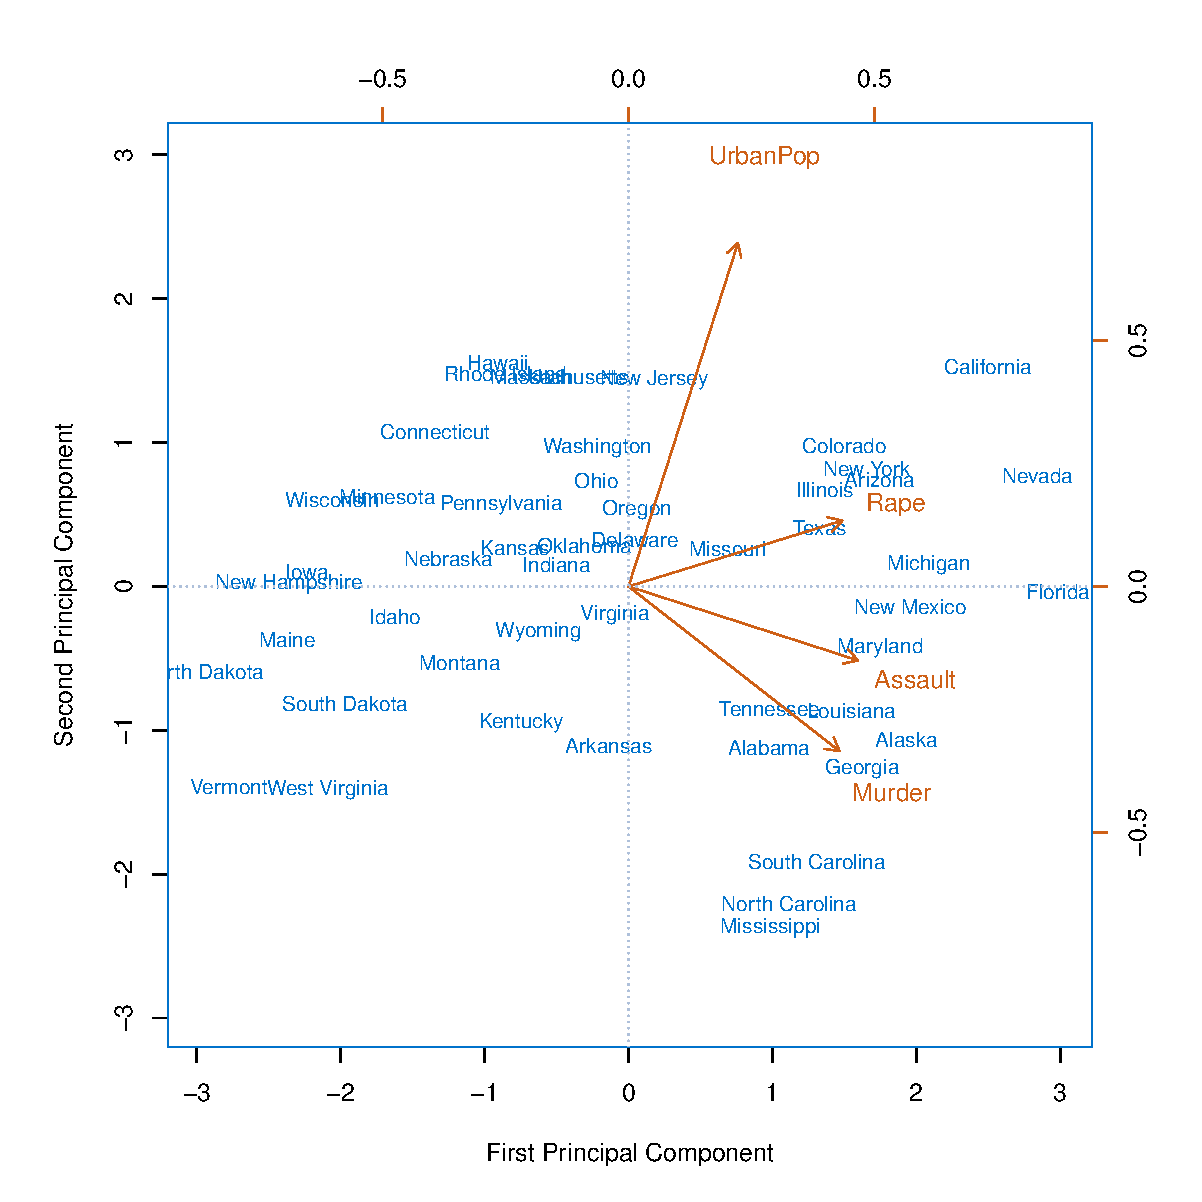
\includegraphics[width=\textwidth]{../class11/Figures_Chapters_7-13/Chapter12/12_1.pdf} \\

\scriptsize Source: ISLR2 Figure 12.1
\end{column}
\end{columns}
\end{frame}

\begin{frame}{PCA -- Technicalities}
\begin{itemize}
  \item Each PC is an \textbf{eigenvector} of the data correlation matrix:
\begin{align*}
V^{-1}CV = \Lambda
\end{align*}
 where $V$ are the eigenvectors, $C$ is the correlation matrix, and $\Lambda$ is a diagonal matrix of eigenvalues
\end{itemize}
\begin{itemize}
  \item The \textbf{proportion of variance explained} $f_k$ by each PC $k$ is proportional to the corresponding \textbf{eigenvalue} $\lambda_k$:
\begin{align*}
f_k = \frac{\lambda_k}{\sum_{j=1}^p \lambda_{j}} 
\end{align*}
  \item The cumulative proportion of variance $F_k$ explained by the first $k$ PC is then:
\begin{align*}
F_k = \frac{\sum_{j=1}^k \lambda_j}{\sum_{j'=1}^p \lambda_{j'}}
\end{align*}
\end{itemize}
\end{frame}

\begin{frame}{PCA -- Screeplot \small [cont'd]}
\begin{block}{Choosing the Number of Principal Components}
\small
\begin{itemize}
   \item Eigenvalue $\lambda > 1$
   \item Cumulative explained variance greater than threshold
   \item Cross-validation to find optimal $K$ (lowest test error) in a linear regression or classification model
   \item ''Eyeballing'' the screeplot
\end{itemize}
\end{block}
\centering
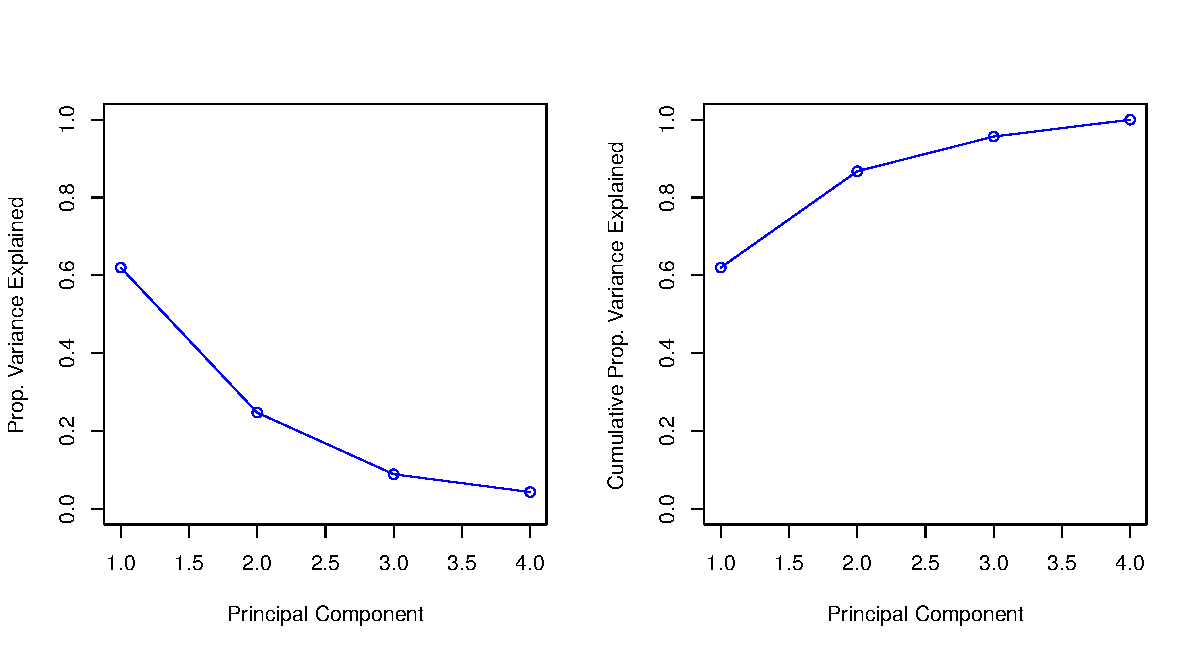
\includegraphics[width=.8\textwidth]{../class11/Figures_Chapters_7-13/Chapter12/12_3.pdf} \\

\scriptsize Source: ISLR2 Figure 12.3
\end{frame}

\begin{frame}[fragile]{PCA in R}
Use the \texttt{USArrests} dataset that contains data on the arrests (per 100,000 residents) for various violent crimes as well as the percentage of urban population in the 50 states of the US.
\begin{Rcode}
?USArrests
summary(USArrests)

# PCA using prcomp()
# Scaling is generally a good idea
pca.result <- prcomp(USArrests, scale=TRUE)

# Print the component loadings
pca.result$rotation

# Biplot for components 1 and 2
biplot(pca.result, scale=0)

# Explained variance for each component
pca.result$sdev^2
# Scree plot (both points and lines)
plot(pca.result$sdev^2, type='b')
\end{Rcode}
\end{frame}

\begin{frame}{PCA in R \small [cont'd]}
Biplot and Screeplot: \\

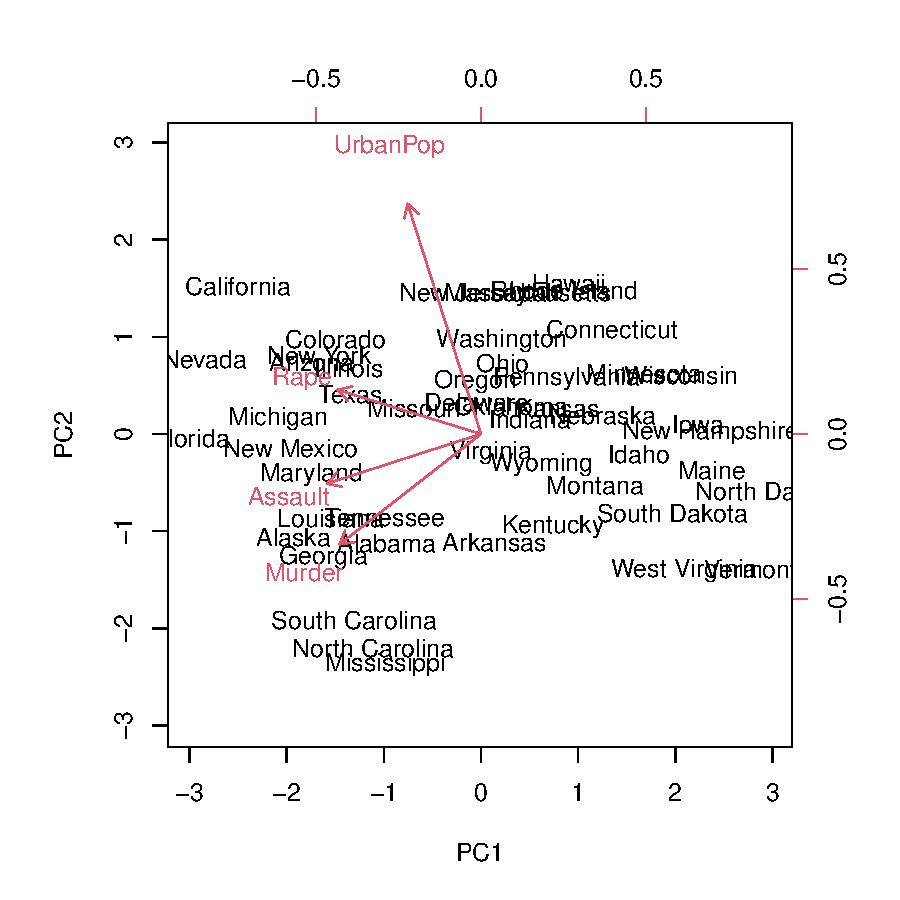
\includegraphics[width=.49\textwidth]{biplot.pdf}
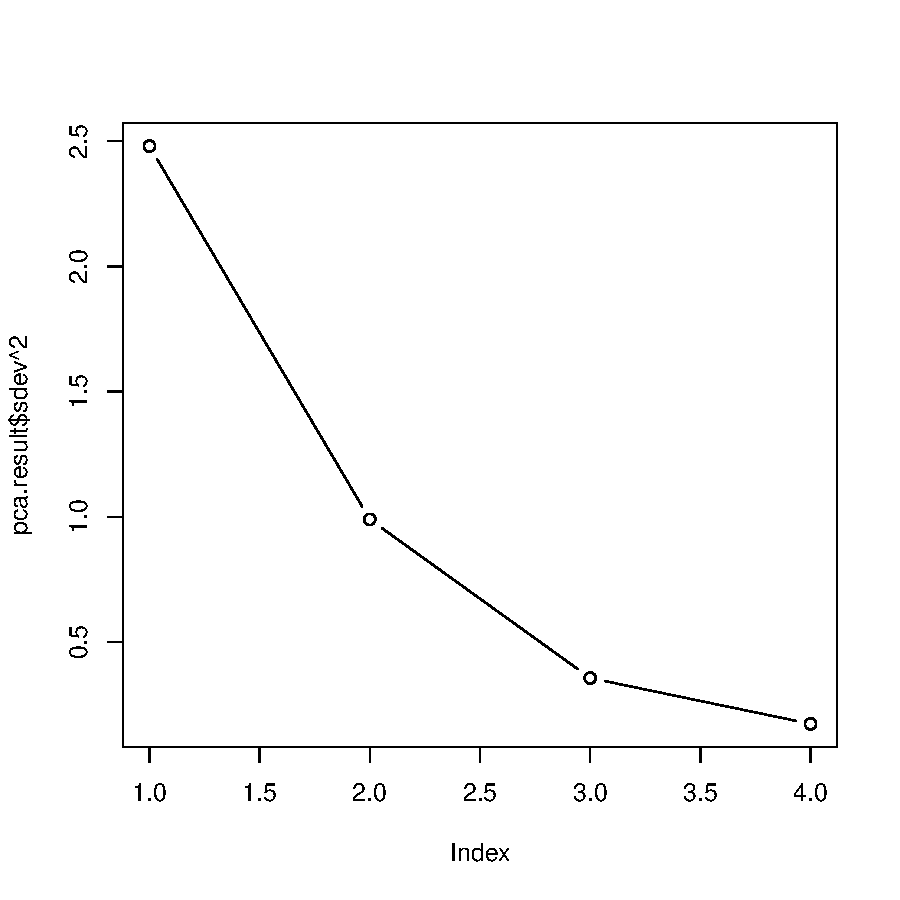
\includegraphics[width=.49\textwidth]{screeplot.pdf}
\end{frame}

\begin{frame}[fragile]{PCA in R \small [cont'd]}
continued \ldots
\begin{Rcode}
# Proportion of variance explained
pve <- pca.result$sdev^2 / sum(pca.result$sdev^2)

# Cumulative sum of variance explained
plot(cumsum(pve), type='b')

# Eigen-decomposition of correlation matrix
e <- eigen(cor(USArrests))
# Compare values and vectors to prcomp results
e$values
e$vectors

# Print the component scores themselves
# For further use in regression, etc.
head(pca.result$x)
\end{Rcode}
\end{frame}

\begin{frame}{Hands-On Exercises -- PCA}
The \texttt{Boston} dataset in the \texttt{ISLR2} library describes house prices in the different suburbs of Boston. Use PCA to reduce the number of dimensions for this dataset:
\begin{enumerate}
   \item Use the \texttt{prcomp} function to perform a PCA on the centered and standardized data. Limit yourself to quantitative inputs.
   \item Produce a biplot of the first two components
   \item Provide the proportion of variance explained by each component
   \item How many components would you retain? Why? How much of the total variance would this explain?
   \item Based on the loadings, can you ascribe meaning to the components? What do they represent?
\end{enumerate}
\end{frame}

\begin{frame}{Hands-On Exercises -- PCA}
The \texttt{Harmann74.cor} dataset in the \texttt{datasets} library contains the results of 24 psychological tests given to 145 school children. 
Use PCA to reduce the number of dimensions for this dataset:
\begin{enumerate}
   \item Use the \texttt{prcomp} function to perform a PCA on the centered and standardized data. Limit yourself to quantitative inputs.
   \item Produce a biplot of the first two components
   \item Provide the proportion of variance explained by each component
   \item How many components would you retain? Why? How much of the total variance would this explain?
   \item Based on the loadings, can you ascribe meaning to the components? What do they represent?
\end{enumerate}
\end{frame}

\begin{frame}{Hands-On Exercises -- PCA}
The \texttt{Hitters} dataset in the \texttt{ISLR2} library contains the salary of 322 baseball players and season statistics. Use \texttt{salary} as the target variable and all other numerical variables as predictors. 

\begin{enumerate}
   \item Use PCA to reduce the number of dimensions for the predictors.
   \item Retain the first principal component.
   \item Estimate and cross-validate a regression model using the first PC as predictor. What is the training and validation error?
   \item Repeat steps (1) to (3), retaining 2, 3, \ldots, all components
   \item Plot the training and validation error agains the number of components. Describe and discuss your results.
\end{enumerate}
\end{frame}


\begin{frame}{Clustering}
\begin{block}{Goals}
\begin{itemize}
   \item Form homogenous subgroups of data
   \item Based on \emph{similarity} of (or \emph{distance} between) observations
   \item Discover ''structure'' in the data
   \item Clustering observations based on features, or clustering features based on observations (transpose of data matrix)
\end{itemize}
\end{block}
\begin{block}{K-Means Clustering}
\begin{itemize}
   \item Number of clusters $K$ is given 
\end{itemize}
\end{block}
\begin{block}{Hierarchical Clustering}
\begin{itemize}
   \item Unknown or variable number of clusters
\end{itemize}
\end{block}
\end{frame}

\begin{frame}{K-Means Clustering}
\begin{itemize}
  \item Minimize within-cluster variation $W(C_i)$:
\begin{align*}
\min_{C_i} \left\{ \sum_{k=1}^K W(C_k) \right\}
\end{align*}
  \item Squared Euclidean Distance
  \begin{itemize}
     \item Between every pair of observations in the cluster (equation \ref{eq:1})
     \item Between every observation and the cluster \textbf{centroid} (''mean'') (equation \ref{eq:2})
  \end{itemize}
\begin{align}
W(C_k) &= \frac{1}{|C_k|} \sum_{i,i' \in C_k} \sum_{j=1}^p (x_{ij} - x_{i'j})^2 \label{eq:1} \\
&= 2 \sum_{i \in C_k} \sum_{j=1}^p (x_{ij} - \bar{\mu}_{kj})^2 \label{eq:2}
\end{align}
  \item Only for quantitative variables
\end{itemize}
\end{frame}

\begin{frame}{K-Means Clustering}
\centering
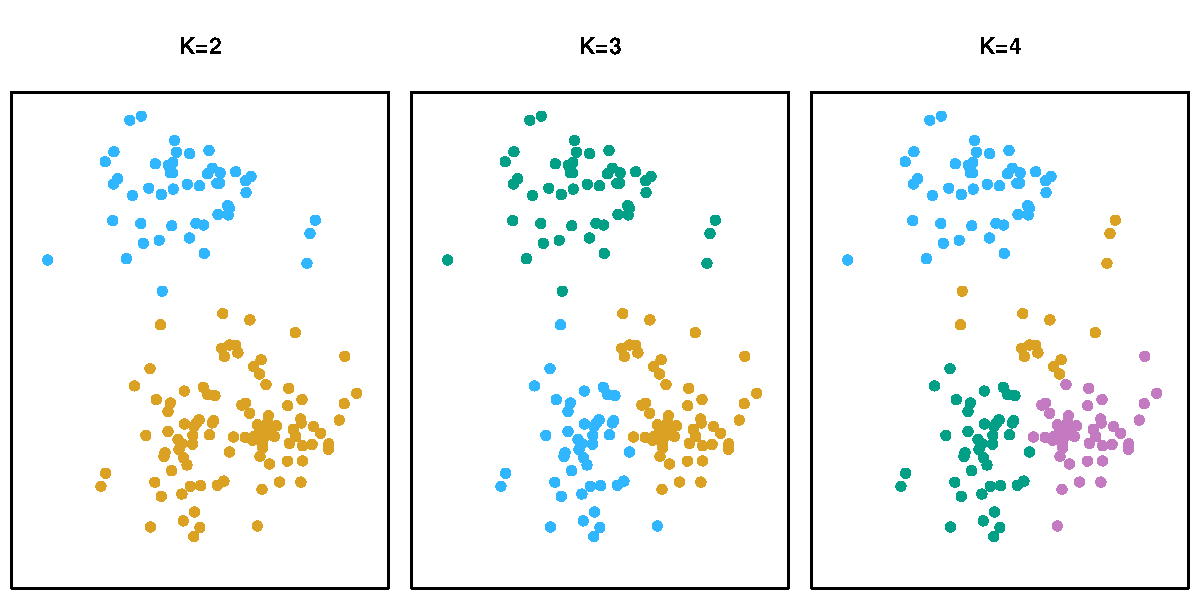
\includegraphics[width=\textwidth]{../class11/Figures_Chapters_7-13/Chapter12/12_7.pdf} \\

\scriptsize Source: ISLR2 Figure 12.7
\end{frame}

\begin{frame}{K-Means Clustering -- Iterative Cluster Assignment}
\begin{columns}
\begin{column}{0.35\textwidth}
\small
\begin{enumerate}
   \item Randomly assign each observation to a cluster
   \item Iterate until cluster assignments are stable
   \begin{enumerate}
       \small
       \item Compute cluster means / centroid
       \item Assign each observation to cluster with closest centroid
   \end{enumerate}
\end{enumerate}
\end{column}
\begin{column}{0.65\textwidth}
\centering
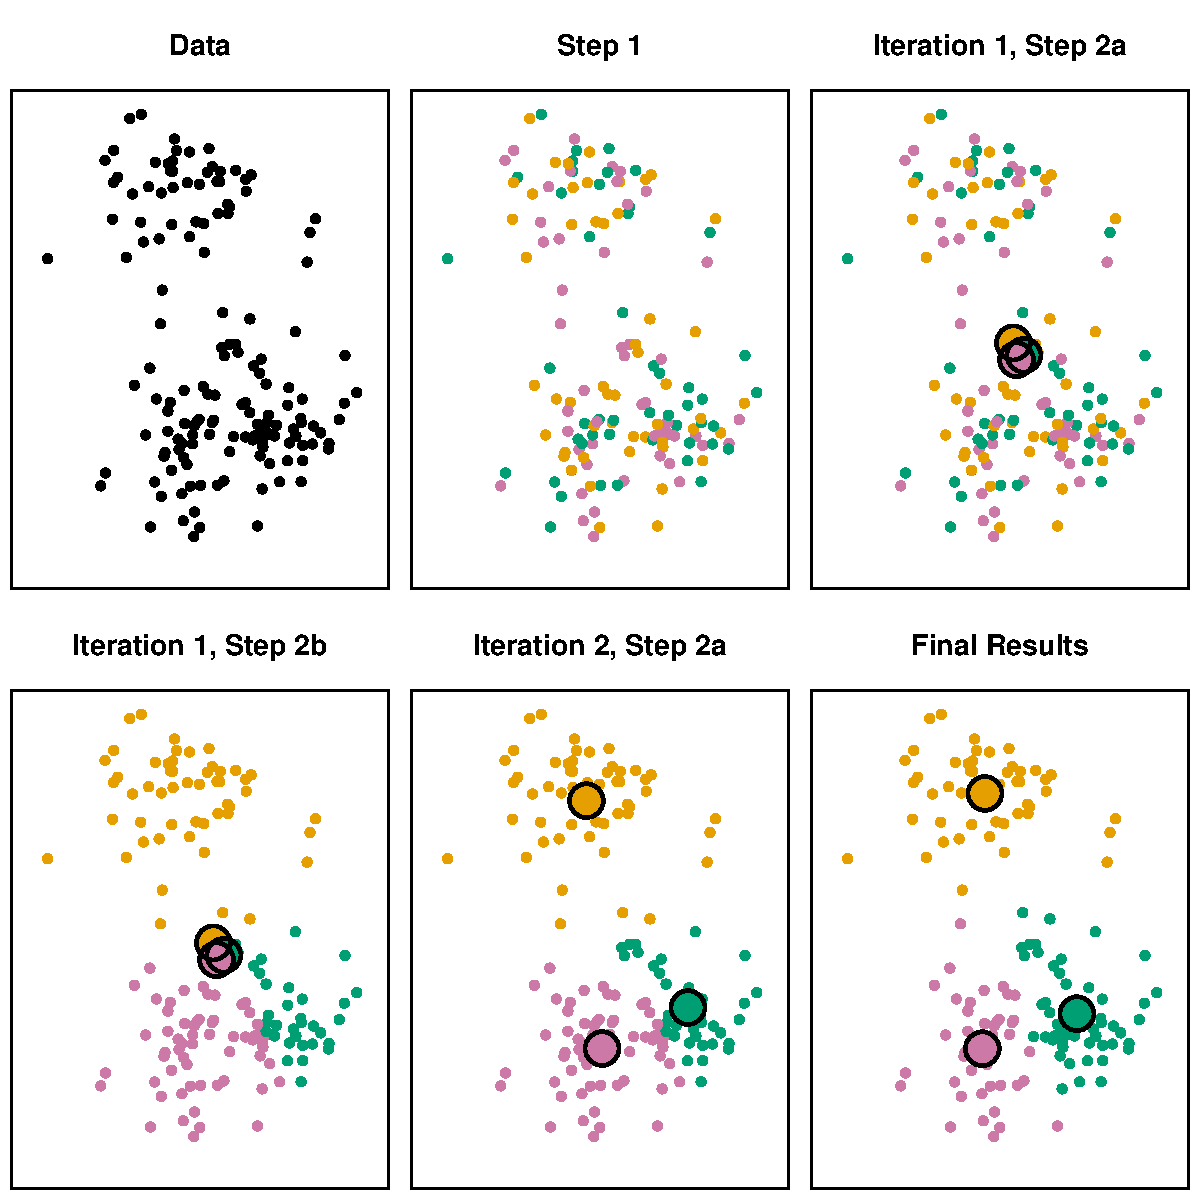
\includegraphics[width=\textwidth]{../class11/Figures_Chapters_7-13/Chapter12/12_8.pdf} \\

\scriptsize Source: ISLR2 Figure 12.8
\end{column}
\end{columns}
\end{frame}

\begin{frame}{K-Means Clustering -- Randomized Starting}
\begin{columns}
\begin{column}{0.35\textwidth}
\begin{itemize}
   \item Different random initial starting clusters lead to different (suboptimal) solutions 
   \item Run algorithm multiple times and select solution with lowest objective value
\end{itemize}
\end{column}
\begin{column}{0.65\textwidth}
\centering
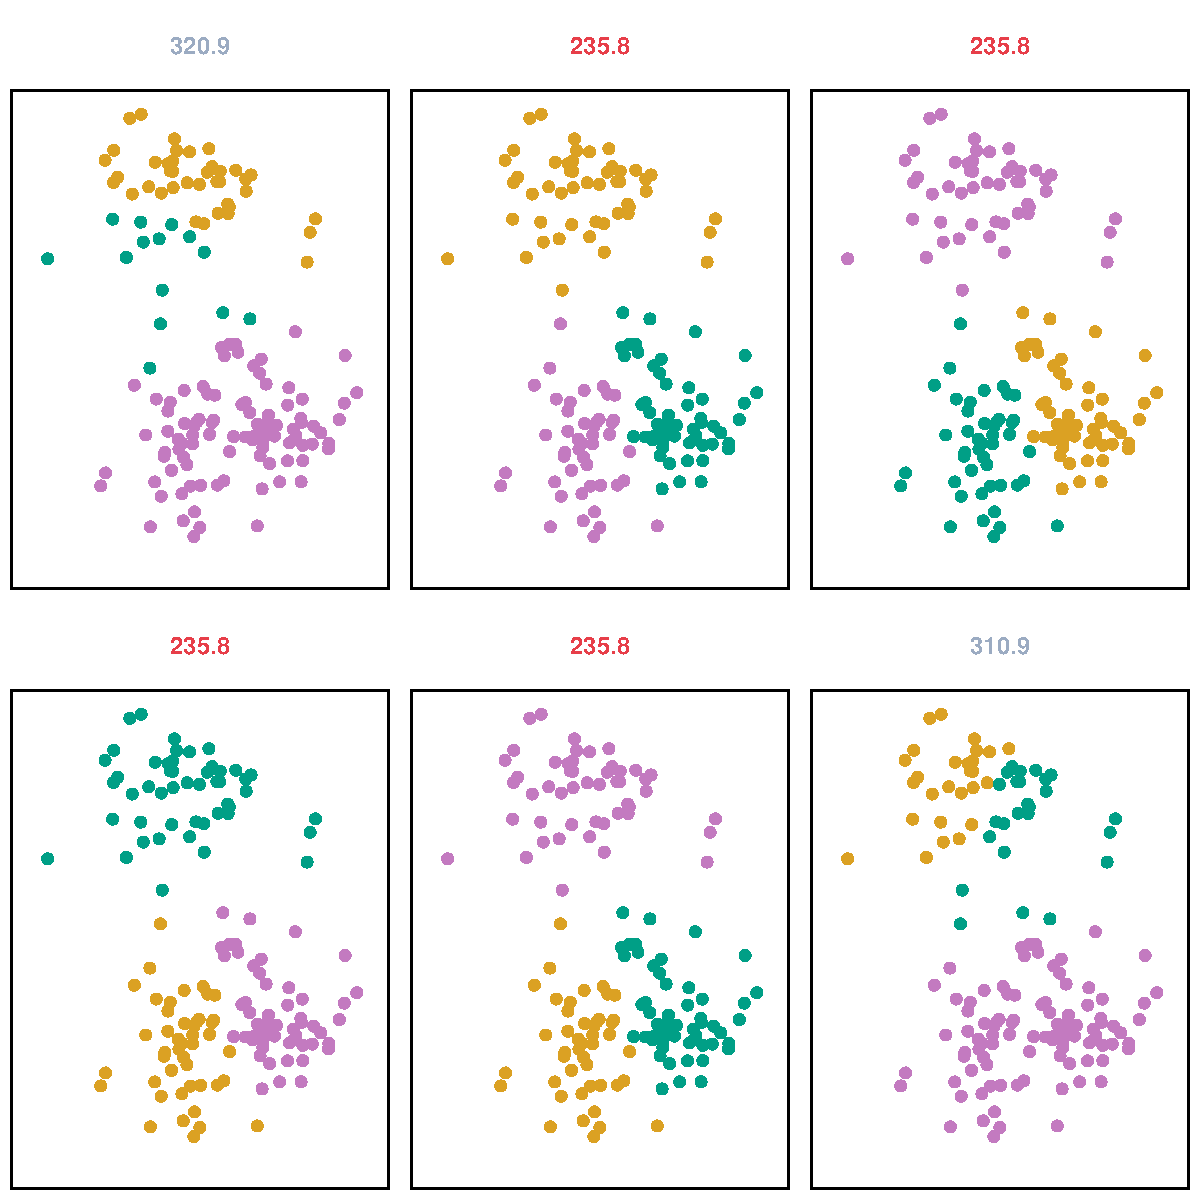
\includegraphics[width=\textwidth]{../class11/Figures_Chapters_7-13/Chapter12/12_9.pdf} \\

\scriptsize Source: ISLR2 Figure 12.9
\end{column}
\end{columns}
\end{frame}

\begin{frame}[fragile]{K-Means Clustering in R}
Simulated example:
\begin{Rcode}
# Set RNG seed for replicability
set.seed(2)

# Create a 50 x 2 matrix of random variables 
# Normally distributed, with 0 mean and SD=1
x <- matrix(rnorm(n=50*2, mean=0, sd=1), ncol=2)

# Clearly separate the first 25 points by
# shifting their coordinates
x[1:25, 1] <- x[1:25, 1] + 3
x[1:25, 2] <- x[1:25, 2] - 4

# Cluster into 2 clusters, performing
# 20 random starting assignments
km.result <- kmeans(x, 2, nstart=20)
\end{Rcode}
\end{frame}

\begin{frame}[fragile]{K-Means Clustering in R \small [cont'd]}
continued \ldots
\begin{Rcode}
# Results show cluster means, cluster
# assignments, and sums of squares (distances)
# within and between 
km.result
# Those values are also available in
# the result object
names(km.result)

# Plot the color-coded points
plot(x, col=(km.result$cluster+1),
     main = 'K-Means Clustering Results with K=2',
     xlab = '', ylab='', pch=20, cex=2)
\end{Rcode}
\end{frame}

\begin{frame}{K-Means Clustering in R \small [cont'd]}
\centering

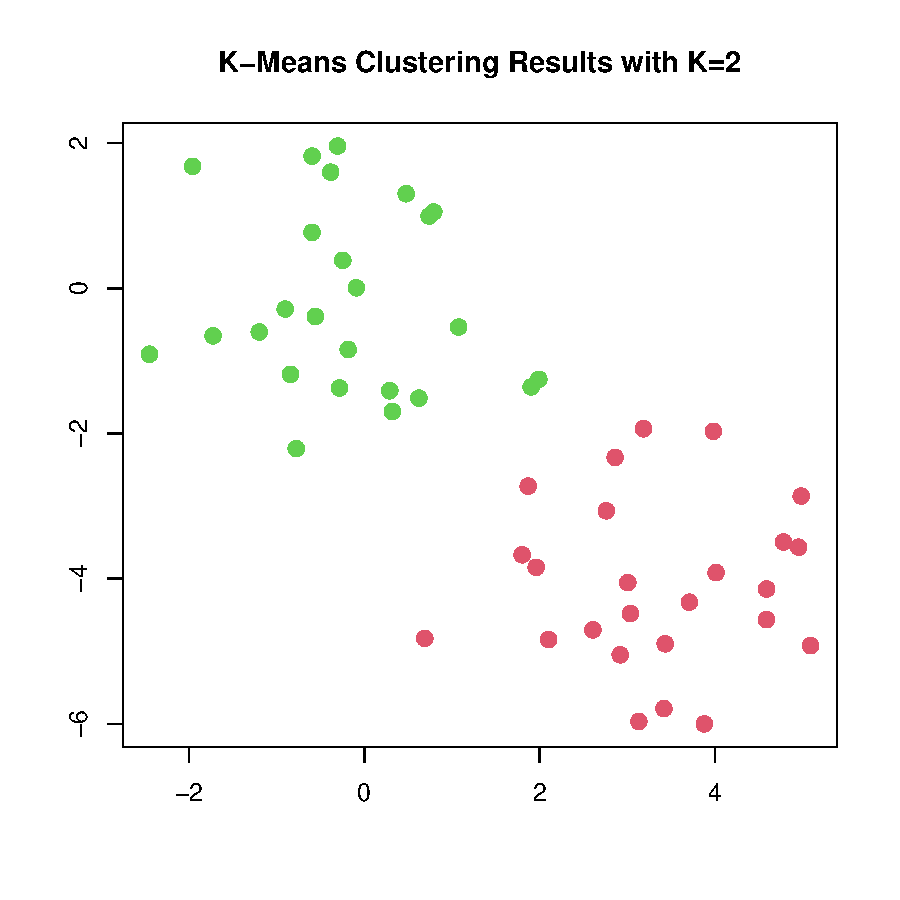
\includegraphics[height=3in]{kmeans.pdf}
\end{frame}

\begin{frame}{Hands-On Exercises -- K-Means Clustering}
The \texttt{Boston} dataset in the \texttt{ISLR2} library describes house prices in the different suburbs of Boston. Use K-Means Clustering to identify sets of similar suburbs using only the numerical variables in the data set.
\begin{enumerate}
   \item Use the \texttt{kmeans} function to perform a cluster analysis, using multiple starting assignments. Limit yourself to quantitative inputs.
   \item Use different numbers of clusters $k$ and identify which value of $k$ gives you the best results. Justify your choice.
   \item Scale the data so that each variable has the same variance or standard deviation, but do not change the variable means. 
   \item Repeat the cluster analysis with the best value of $k$ and compare results.\end{enumerate}
\end{frame}

\begin{frame}{Hands-On Exercises -- K-Means Clustering}
The \texttt{Hitters} dataset in the \texttt{ISLR2} library contains the salary of 322 baseball players and season statistics. Use K-Means Clustering to identify sets of similar players, using only the numerical variables in the data set.

\begin{enumerate}
   \item Use the \texttt{kmeans} function to perform a cluster analysis, using multiple starting assignments. Limit yourself to quantitative inputs.
   \item Use different numbers of clusters $k$ and identify which value of $k$ gives you the best results. Justify your choice.
   \item Scale the data so that each variable has the same variance or standard deviation, but do not change the variable means. 
   \item Repeat the cluster analysis with the best value of $k$ and compare results.\end{enumerate}
\end{frame}

\begin{frame}{Hierarchical Clustering}
\begin{block}{Bottom-Up / Agglomerative Clustering}
\begin{enumerate}
   \item Begin with $n$ observations and a dissimilarity or distance metric
   \item Treat each observation as its own cluster
   \item Repeat $n-2$ times:
   \begin{enumerate}
      \normalsize
      \item Calculate dissimilarities or distances between all pairs of clusters
      \item Identify the pair of clusters that are least dissimilar (most similar)
      \item ''Fuse'' or merge these two clusters
   \end{enumerate}
\end{enumerate}
\end{block}
\end{frame}

\begin{frame}{Hiearchical Clustering}
\begin{block}{Dendrogram}
\begin{itemize}
  \item Shows what clusters were fused at what dissimilarity
\end{itemize}
\end{block}
\centering
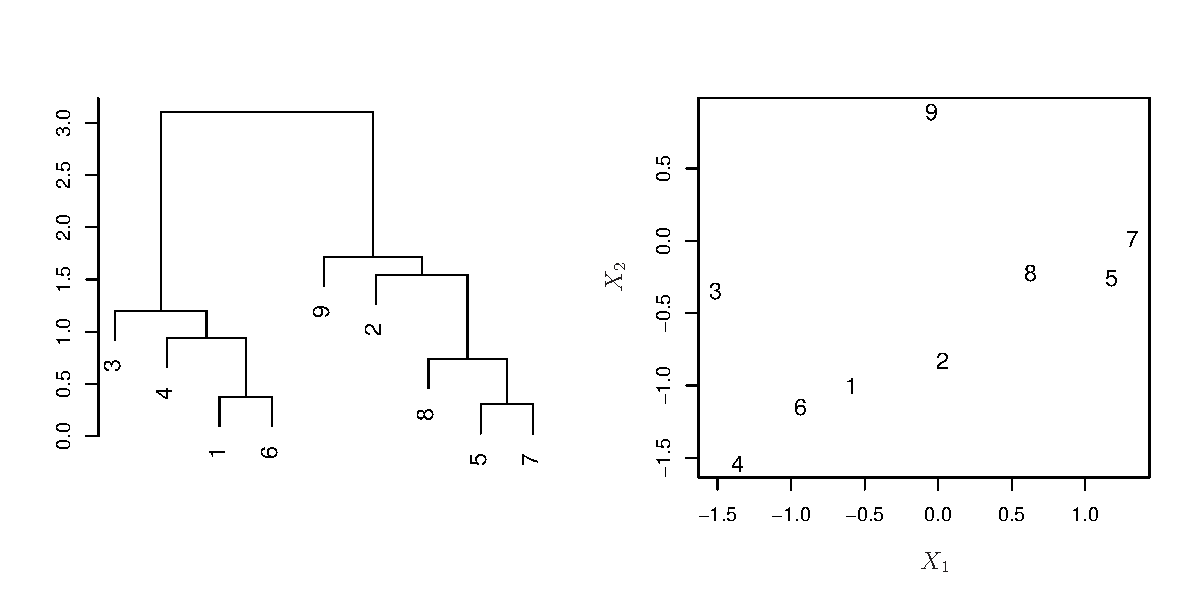
\includegraphics[width=\textwidth]{../class11/Figures_Chapters_7-13/Chapter12/12_12.pdf} \\

\scriptsize Source: ISLR2 Figure 12.12
\end{frame}

\begin{frame}{Hierarchical Clustering}
\begin{block}{Key Decisions}
\begin{itemize}
   \item How to measure dissimilarity/distance between observations?
   \item How to measure dissimilarity between clusters (''\textbf{linkage}'')?
   \item How many clusters should we have?
\end{itemize}
\end{block}
\end{frame}


\begin{frame}{Hierarchical Clustering -- Common Distance Metrics}
\begin{block}{Common Distance Metrics or ''Norms''}
\renewcommand{\arraystretch}{2}
\centering 
\footnotesize
\begin{tabular}{l|c|c} \hline
\begin{minipage}{1.75cm}Taxicab / Manhattan\end{minipage} & $ ||q-p||_1 $ & $\displaystyle \sum_i | q_i - p_i |$ \\ \hline
Euclidean & $ ||q-p||_2$ & $\displaystyle \sqrt{ \sum_i (q_i-p_i)^2}$ \\ \hline
Minkowski & $||q-p||_p$ & $\displaystyle \left( \sum_i | q_i - p_i |^p \right)^{\frac{1}{p}}$ \\ \hline
Chebyshev & $||q-p||_\infty$ & $\displaystyle \lim_{p \rightarrow \infty} \left( \sum_i | q_i - p_i |^p \right)^{\frac{1}{p}} = \max_i( | q_i - p_i | )$ \\ \hline
  & $||q-p||_{-\infty}$ & $\displaystyle \lim_{p \rightarrow -\infty} \left( \sum_i | q_i - p_i |^p \right)^{\frac{1}{p}} = \min_i( | q_i - p_i | )$ \\ \hline
\end{tabular}
\end{block}
\end{frame}

\begin{frame}{Hierarchical Clustering -- Common Distance Metrics}
\centering
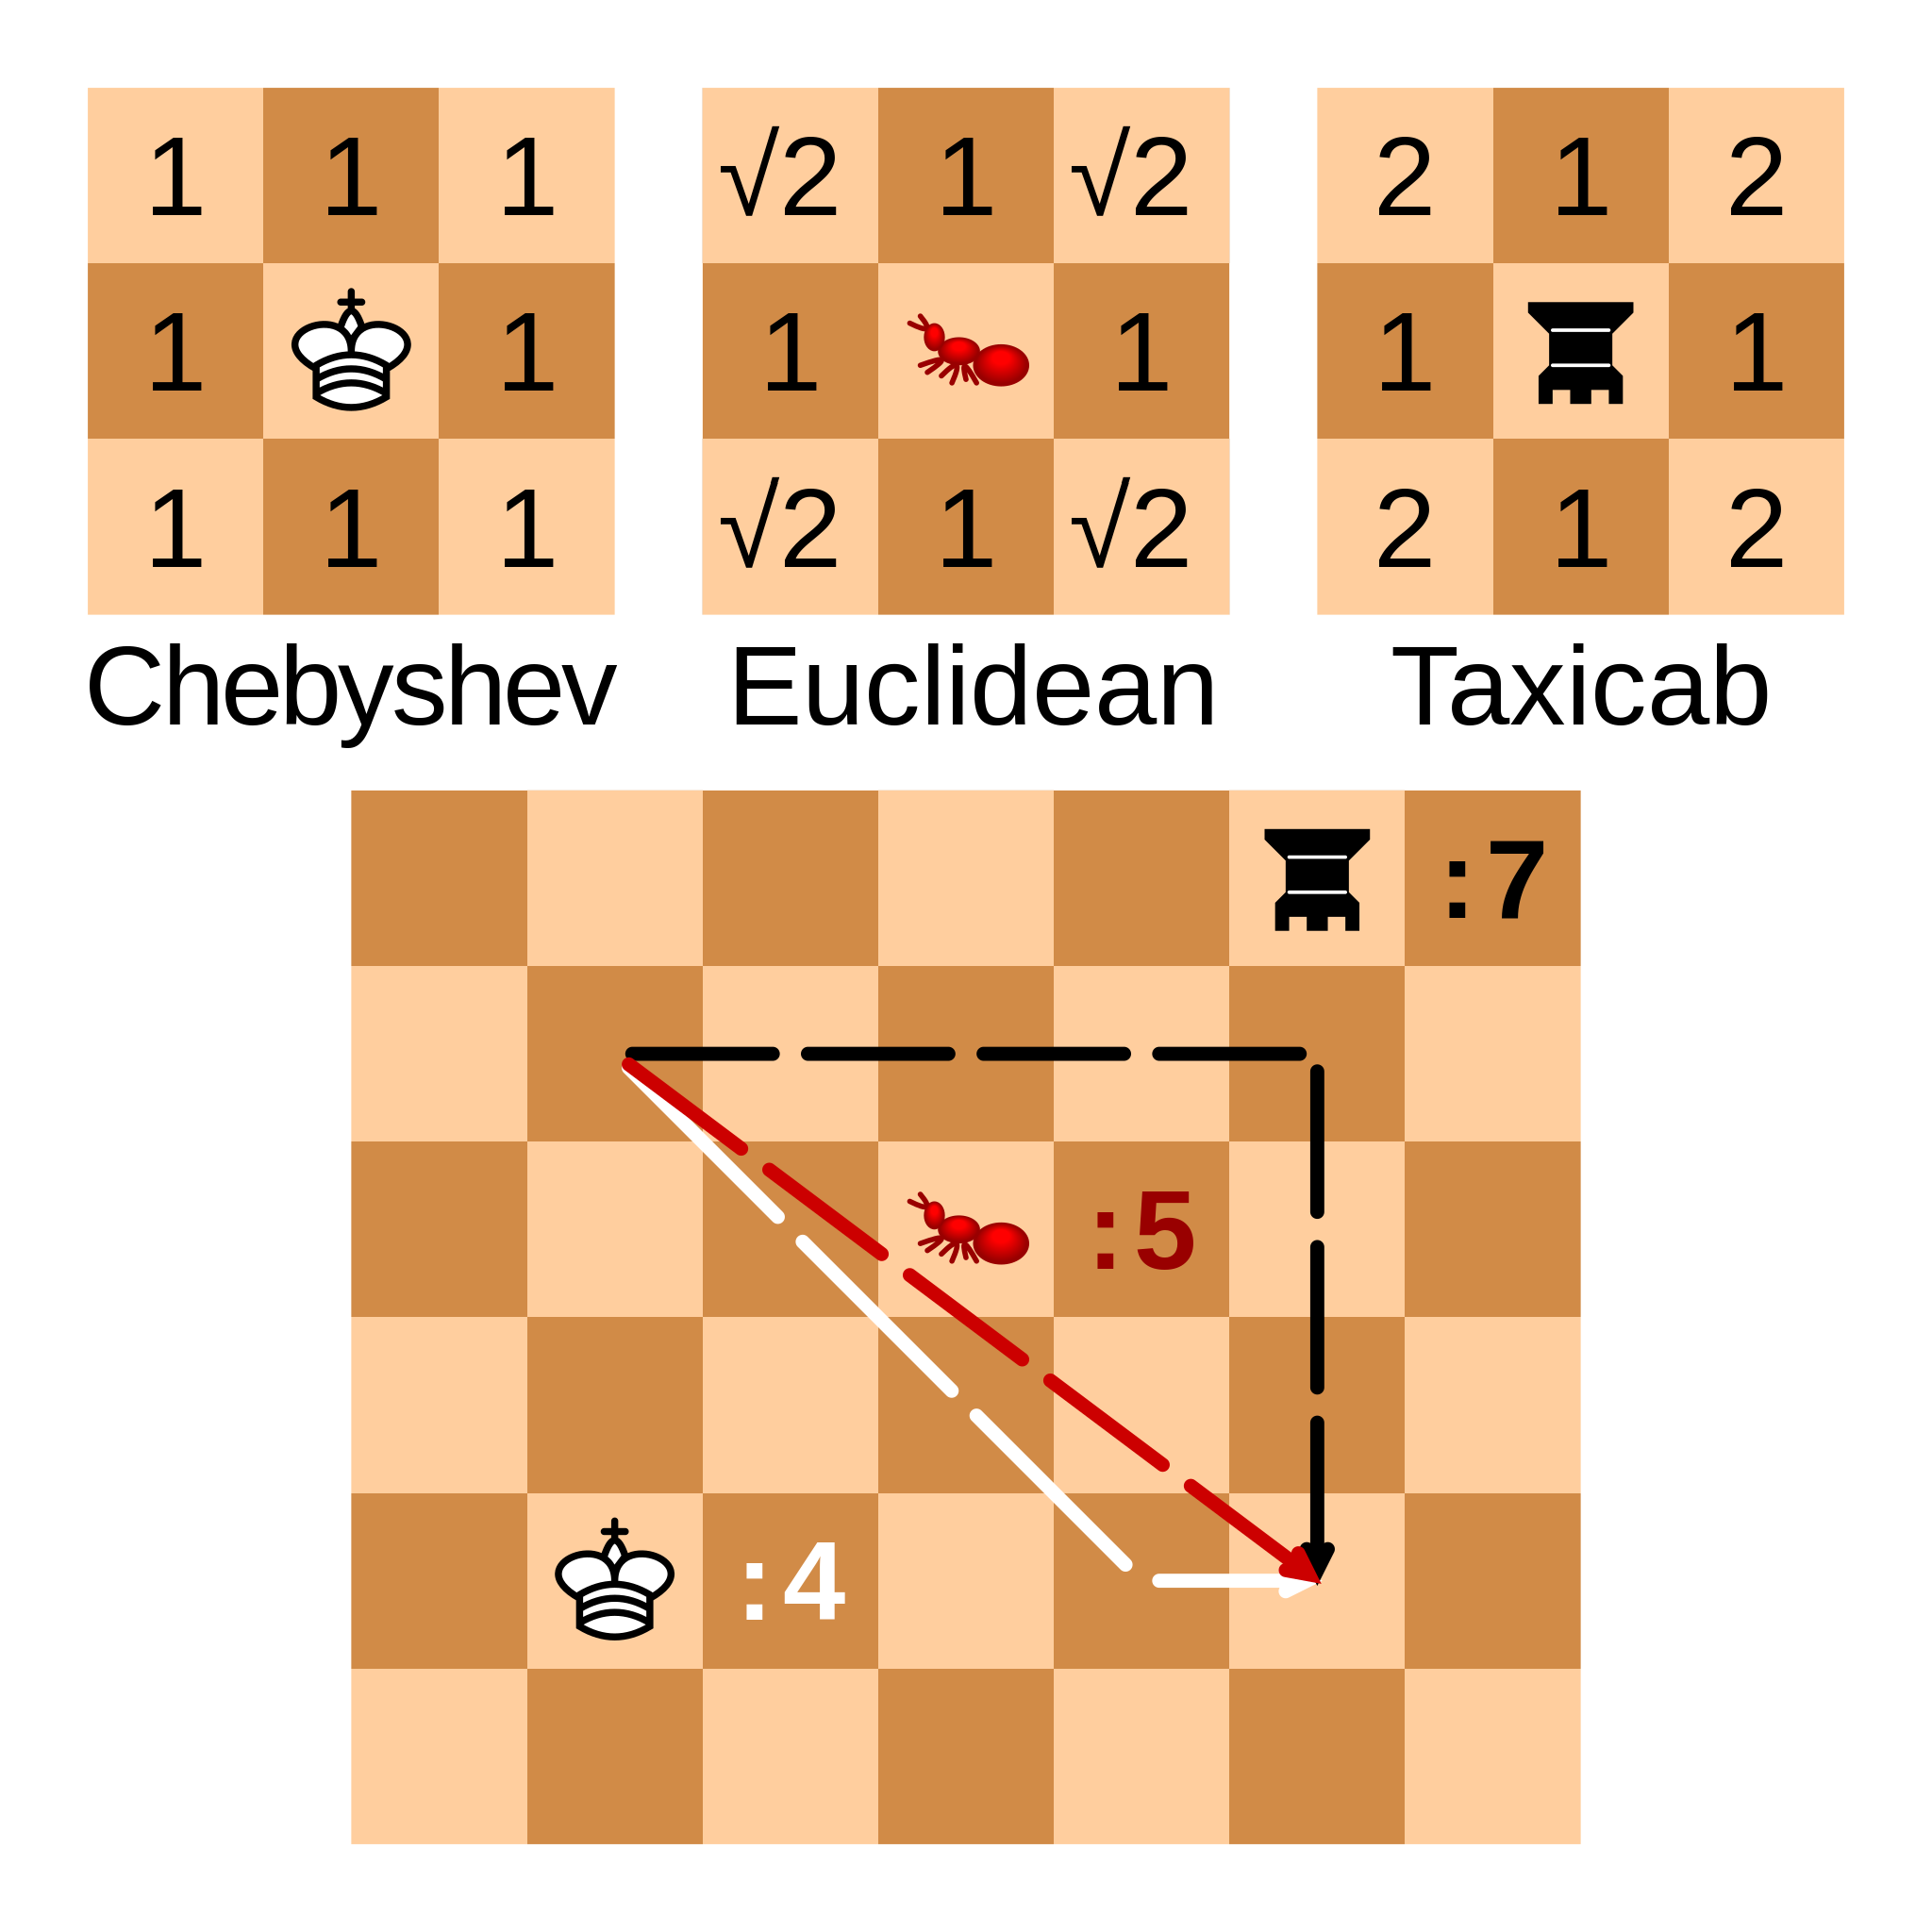
\includegraphics[height=3in]{Minkowski_distance_examples.svg.png} \\

\scriptsize \url{https://commons.wikimedia.org/wiki/File:Minkowski_distance_examples.svg}
\end{frame}

\begin{frame}{Hierarchical Clustering -- Common Linkage Criteria}
\begin{block}{Common Linkages}
\renewcommand{\arraystretch}{1.5}
\centering

\begin{tabular}{l|l} \hline
Single & $\displaystyle d_{SL}(G,H) = \min_{i \in G, i' \in H} d_{i, i'}$  \\ \hline
Complete & $\displaystyle d_{CL}(G,H) = \max_{i \in G, i' \in H} d_{i, i'}$  \\ \hline
Average & $\displaystyle d_{AL}(G,H) = \operatorname*{mean}_{i \in G, i' \in H} d_{i, i'}$  \\ \hline
\end{tabular}
\end{block}
\small
\vspace{\baselineskip}
There are many other linkage functions: \url{https://en.wikipedia.org/wiki/Hierarchical_clustering}
\end{frame}

\begin{frame}{Hierarchical Clustering -- Common Linkage Criteria}
\centering
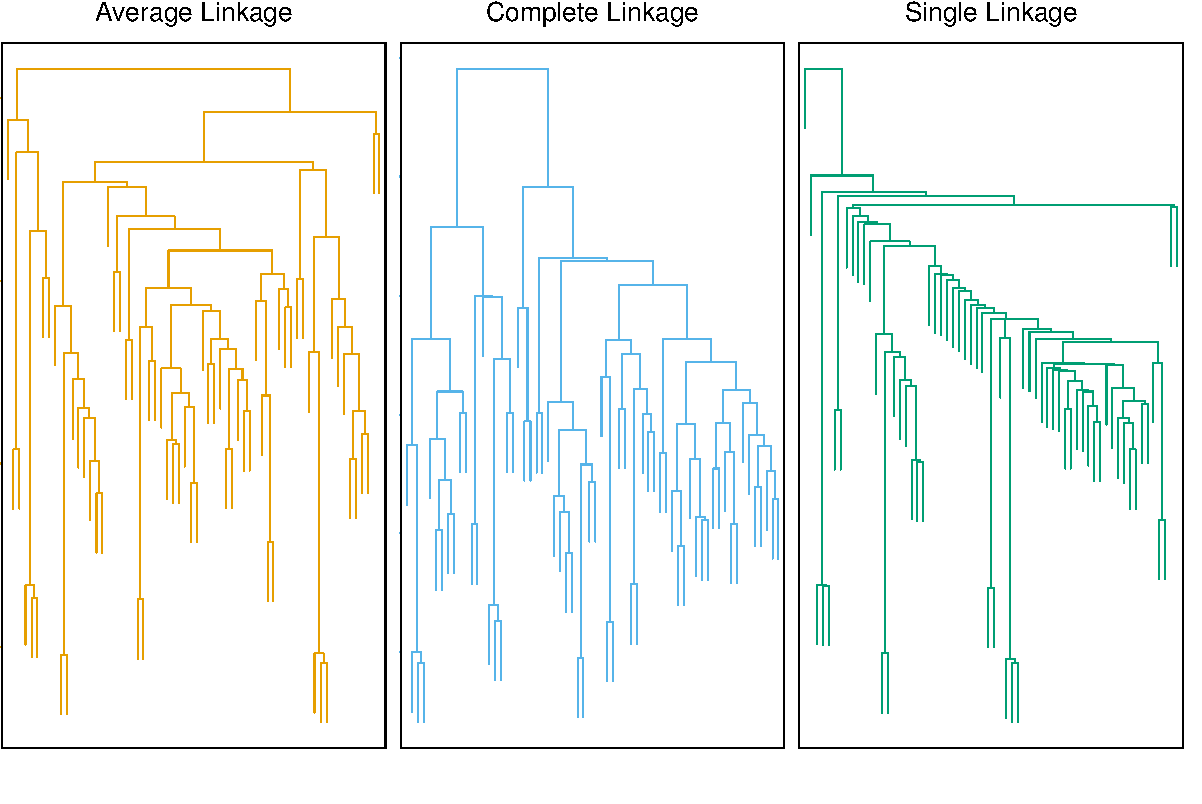
\includegraphics[width=\textwidth]{../class11/Figures_Chapters_7-13/Chapter12/12_14.pdf} \\

\scriptsize Source: ISLR2 Figure 12.14
\end{frame}
\begin{frame}{Hierarchical Clustering -- How Many Clusters?}
\begin{itemize}
  \item ''Cut'' the dendrogram at a dissimilarity value
\end{itemize}

\centering
\vspace{\baselineskip}
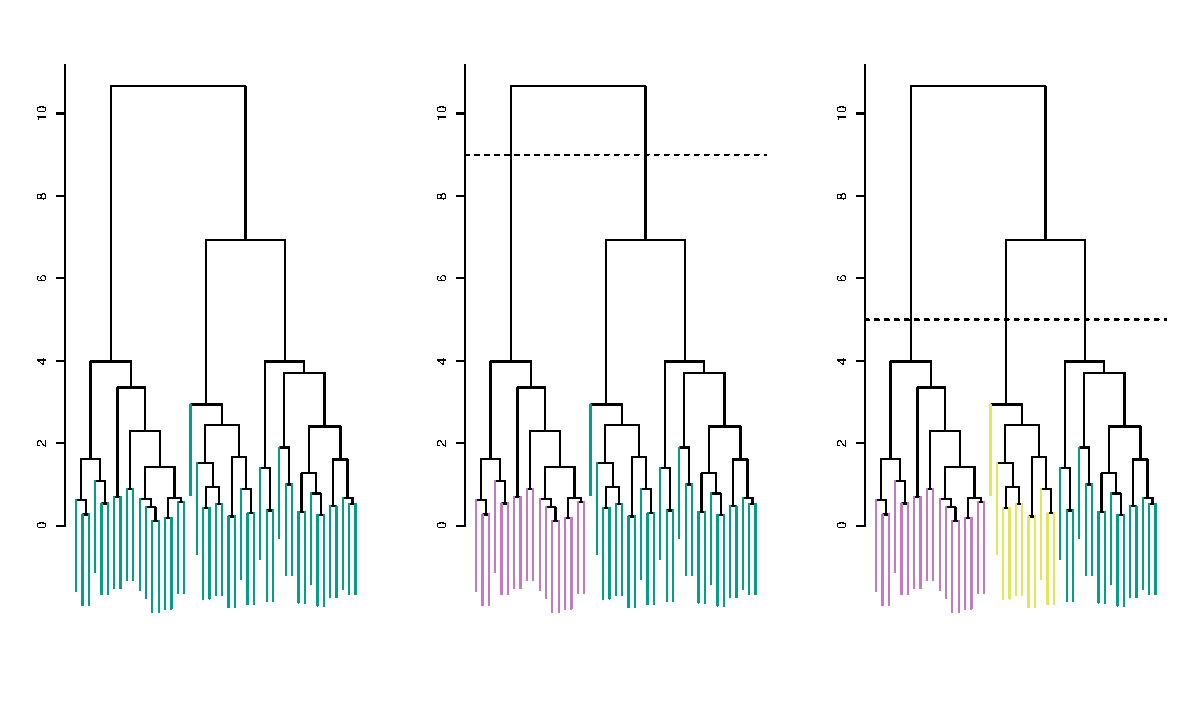
\includegraphics[width=\textwidth]{../class11/Figures_Chapters_7-13/Chapter12/12_11.pdf} \\

\scriptsize Source: ISLR2 Figure 12.11
\end{frame}

\begin{frame}[fragile]{Hierarchical Clustering in R}
\begin{Rcode}
# The dist() function calculated distances
# according to a variety of metrics/norms
euclid.dist <- dist(x, method='euclidean')
pnorm.dist <- dist(x, method='minkowski', p=3)
manh.dist <- dist(x, method='manhattan')
max.dist <- dist(x, method='maximum')

# Use the hclust() function with a distance metric
hc.complete <- hclust(euclid.dist, method='complete')
hc.single <- hclust(euclid.dist, method='single')
hc.average <- hclust(euclid.dist, method='average')
\end{Rcode}
\end{frame}

\begin{frame}[fragile]{Hierarchical Clustering in R \small [cont'd]}
continued \ldots
\begin{Rcode}
# Plot the dendrograms in a single plot
par(mfrow = c(1, 3))
plot(hc.complete , col='red', 
   main = "Complete Linkage", 
   xlab = "", sub = "", cex = .9)

plot(hc.average , col='blue', 
   main = "Average Linkage", 
   xlab = "", sub = "", cex = .9)

plot(hc.single , col='green', 
   main = "Single Linkage",
   xlab = "", sub = "", cex = .9)
\end{Rcode}
\end{frame}

\begin{frame}{Hierarchical Clustering in R \small [cont'd]}
\centering
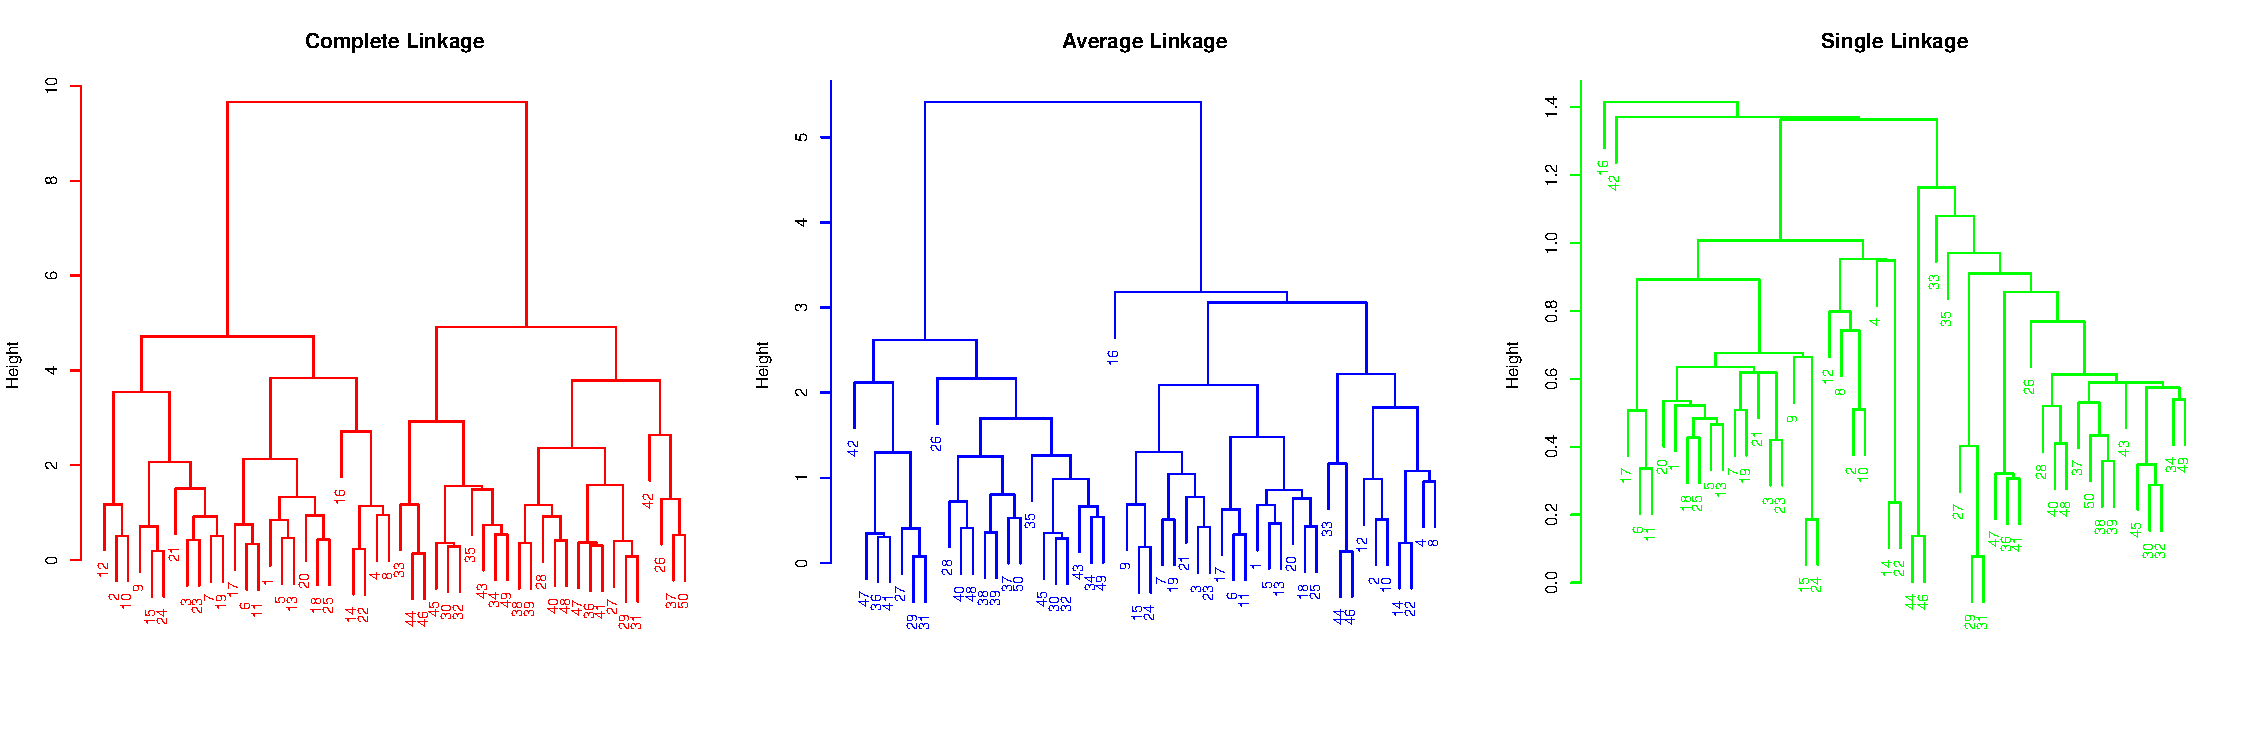
\includegraphics[width=\textwidth]{hclust.pdf}
\end{frame}

\begin{frame}[fragile]{Hierarchical Clustering in R \small [cont'd]}
Cutting the tree and identifying clusters:
\begin{Rcode}
# Cut by number of groups/clusters
cutree(hc.complete, k=4)
# Cut by height (dissimilarity)
cutree(hc.complete, h=6)
\end{Rcode}
\end{frame}

\begin{frame}{Hands-On Exercises -- Hierarchical Clustering}
The \texttt{Boston} dataset in the \texttt{ISLR2} library describes house prices in the different suburbs of Boston. Use Hierarchical Clustering to identify sets of similar suburbs using only the numerical variables in the data set.
\begin{enumerate}
   \item Use the \texttt{hclust} function to perform a cluster analysis, exploring different distance metrics and linkage functions.
   \item Examine the dendrograms and identify which combination of distance metric and linkage function gives you the ''cleanest'' separation of clusters.
   \item How many factors $k$ would you retain?
   \item Using this value for $k$, perform a K-Means Clustering and compare the results.
\end{enumerate}
\end{frame}

\begin{frame}{Hands-On Exercises -- Hierarchical Clustering}
The \texttt{Hitters} dataset in the \texttt{ISLR2} library contains the salary of 322 baseball players and season statistics. Use Hierarchical Clustering to identify sets of similar players, using only the numerical variables in the data set.

\begin{enumerate}
   \item Use the \texttt{hclust} function to perform a cluster analysis, exploring different distance metrics and linkage functions.
   \item Examine the dendrograms and identify which combination of distance metric and linkage function gives you the ''cleanest'' separation of clusters.
   \item How many factors $k$ would you retain?
   \item Using this value for $k$, perform a K-Means Clustering and compare the results.
\end{enumerate}
\end{frame}

\begin{frame}{Hands-On Exercises -- Hierarchical Clustering}
The \texttt{Auto} dataset in the \texttt{ISLR2} library contains information on 392 vehicles. Use Hierarchical Clustering to identify sets of similar vehicles, using only the numerical variables in the data set.

\begin{enumerate}
   \item Use the \texttt{hclust} function to perform a cluster analysis, exploring different distance metrics and linkage functions.
   \item Examine the dendrograms and identify which combination of distance metric and linkage function gives you the ''cleanest'' separation of clusters.
   \item How many factors $k$ would you retain?
   \item Using this value for $k$, perform a K-Means Clustering and compare the results.
\end{enumerate}
\end{frame}


\end{document}

